\documentclass[12pt]{ociamthesis}  % default square logo 
%\documentclass[12pt,beltcrest]{ociamthesis} % use old belt crest logo
%|\documentclass[12pt,shieldcrest]{ociamthesis} % use older shield crest logo

%load any additional packages
\usepackage{amssymb}
\usepackage{url}
\usepackage[toc,page]{appendix}
\usepackage{graphicx}
\graphicspath{{./figures/}}

%============ BIBLIOGRAPHY AND REFS PACKAGES ========%
\usepackage{multibib}
\newcites{x}{References}
\newcites{sec}{Background Reading}

%============ CUSTOM CHAPTER NUMBER ========%

% ============== stuff below is for header\footer
\usepackage{fancyhdr}
\pagestyle{fancy}
\fancyhf{}
\renewcommand{\sectionmark}[1]{\markright{\textit{#1}}}
\renewcommand{\chaptermark}[1]{\markboth{\textsc{#1}}{}}
\fancyhead[R]{\rightmark}
\fancyhead[L]{\leftmark}
\cfoot{\fancyplain{}{\thepage}}

%\makeatletter
%\def\@makechapterhead#1{%
%  \vspace*{50\p@}%
%  {\parindent \z@ \raggedright \normalfont
%    \interlinepenalty\@M
%    \Huge\bfseries  \thechapter.\quad #1\par\nobreak
%    \vskip 40\p@
%  }}
%\makeatother

% ============== FRONT PAGE =========== %
        
\title{Automated Visualised Translation from English to British Sign Language}

\author{Nicolaos Moscholios}             %your name
\college{Pembroke College}  %your college

\degree{Master of Computer Science}     %the degree
\degreedate{Trinity 2016}         %the degree date

%end the preamble and start the document
\begin{document}

%this baselineskip gives sufficient line spacing for an examiner to easily
%markup the thesis with comments
\baselineskip=18pt plus1pt

\maketitle                  % create a title page from the preamble info

\begin{abstract}
A large number of people in the world today are born deaf and many rely on British Sign Language (BSL), the most widely used method of signed communication in the UK. BSL is structured in a completely different way to English and, like any language, it has its own grammar. In order to create a communication bridge between English speakers and individuals affected by deafness there have been attempts at building a formal model of translation. ...
\end{abstract}

\begin{acknowledgements}
I would like to thank...
\end{acknowledgements}

\begin{notes}
The work described in this thesis is available online at \url{nicmosc.com/bsltranslate}. Examples discussed throughout the report marked by an asterisk (*) can be viewed on the website. For demonstrative purposes it is highly suggested that the Examiner try those examples ..
\end{notes}

%\include{abstract}          % include the abstract
{\pagestyle{plain}
	\begin{romanpages}          % start roman page numbering
	%set the number of sectioning levels that get number and appear in the contents
	\setcounter{tocdepth}{5}
	\setcounter{secnumdepth}{5}
	\tableofcontents            % generate and include a table of contents
	\listoffigures              % generate and include a list of figures
	\end{romanpages}            % end roman page numbering
\cleardoublepage}

%===================== CHAPTER 1 ===================%

\chapter{Introduction}
For most people around the world, communication is achieved orally by speaking. Unfortunately some are born deaf or are affected by hearing impairment with time. It is then necessary to use another medium of communication. Today there are about 1 million "functionally deaf" UK individuals \citex{website:bsl-stats}, that is, that require the use of sign language to converse. Additionally there are around 11 million people affected by some degree of hearing loss and while many benefit from hearing aids, sign language bypasses the need to speak, making it easy for everyone to understand each other.  

\section{Motivation}
The problem arises when hearing and Deaf individuals need to communicate. Deaf individuals are taught to read and write English from a young age, but it was found that they have difficulties understanding text with a reading level above that of primary school students \citex{paper:deaf-edu}. Thus it is not enough for hearing individuals to rely on written text to communicate with their community. More and more people are learning BSL even though they have perfectly fine hearing. There are certificates that can be obtained to work with Deaf individuals \citex{website:signature}. Taking lessons from BSL teachers and practising with the community helps to learn the language.

Online resources such as UCL's BSL Sign Bank \citex{website:bsl-sign-bank} and SignBSL.com \citex{website:sign-bsl} offer clips of signers showing words and phrases in BSL for learners and curious people?. The main issue is that they are highly static. Analogously to an English dictionary, it is only useful for looking up individual signs and not \textit{translating} phrases. Research has been carried out to make sign language available to others who rely on spoken English as their primary mean of communication by trying to translate from one language to the other. Although most of the research in the field of automated sign language translation is focussed on ASL, the same concepts apply to BSL, given they are very close since they both originate from English.

Some of those projects went a step further and gave the output as a 3D animation, rather than just a textual representation. Due to the then high computational power necessary to run these systems, none have been made easily available to the public and were just kept as experiments. In 2006, IBM created a fully working system \citex{website:IBM} that allowed users to speak and see the translation from English to BSL in real time; however it has been disregarded and is not obtainable any more. 

\section{Objectives}
This project will aim at creating an online web application that translates from written English to British Sign Language in real time. Through rule-based translation methods (discussed in section \ref{machine translation}) and 3D animation techniques the system will allow users to not only find out what a particular sentence corresponds to in BSL, but also learn and hopefully practice their skills.

\begin{figure}[h]
	\centering
    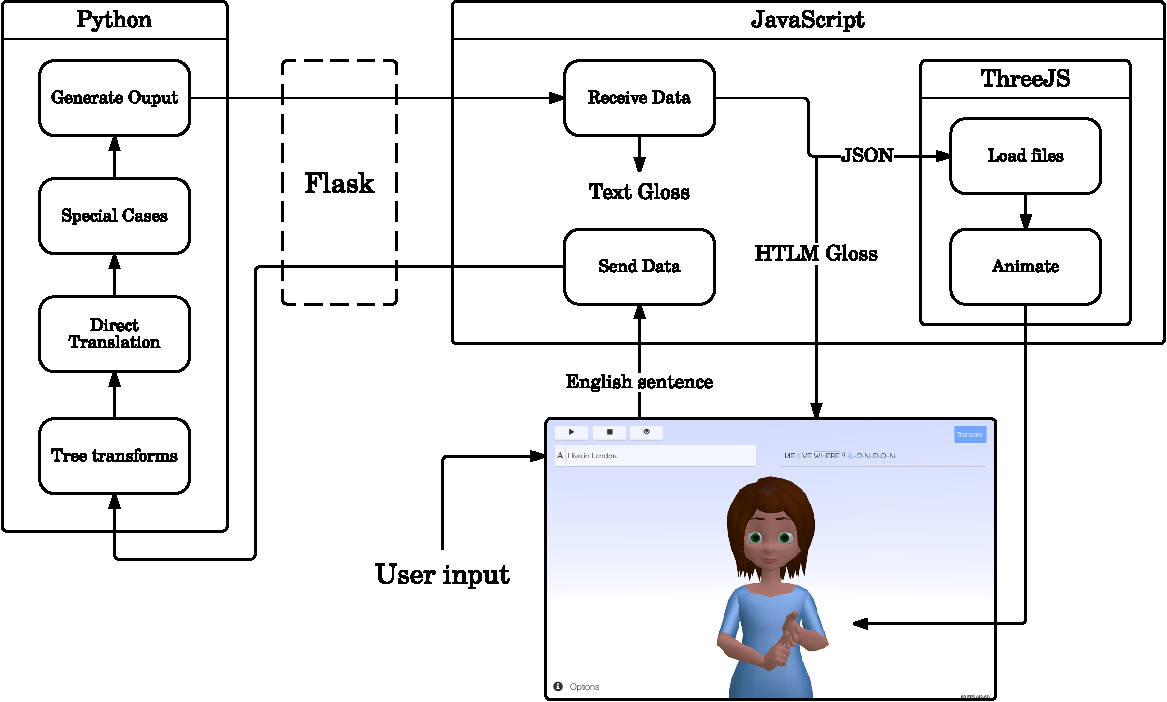
\includegraphics[scale=0.7]{BSL-cropped.pdf}
    \caption{Conceptual overview of the system}
    \label{fig:sys-overview}
\end{figure}

\section{Structure}
The report will read as follows: in chapter 2 we will give a brief introduction to the linguistics British Sign Language and its differences from written English, as well as existing methods of translation from written to written and from written to signed languages. Chapter 3 will cover the design choices for the system, that is, the development environment with the programming languages, the conceptual structure of the pipeline and the end-user interaction. Following up in chapter 4 we explain in detail the implementation of both the translation methods and the animation techniques utilised, as well as the communication between the two modules. Finally chapter 5 will discuss the evaluation of the system both in terms of translation accuracy and feedback from the user survey, while chapter 6 concludes the report along with project achievements, personal remarks and future work.

%===================== CHAPTER 2 ===================%

\chapter{Background}
\section{British Sign Language}
British Sign Language, often shortened to BSL, has been an officially recognised language since 2003 \citex{website:signature}. Like English, it has its own grammar.
\citex{website:deafness} \citex{paper:statistical-SL-MT}
\section{Machine Translation}
\label{machine translation}
\section{Existing Methods}
\section{Personal Work}
\section{Summary}

%===================== CHAPTER 3 ===================%

\chapter{Design}

\section{Language Choice}
\section{Translation}
\section{User Interface}
	\subsection{User Interaction}
\section{Summary}

%===================== CHAPTER 4 ===================%

\chapter{Implementation}

\section{Rule-Based MT in Python}
	\subsection{Pipeline}
	\subsection{System Components}
		\subsubsection{Grammar Tree Transforms}
		\subsubsection{Direct Translation}
		\subsubsection{Special Cases}
		\subsubsection{Output}
	
\section{Animation in ThreeJS}
	\subsection{Blender}
		\subsubsection{Model}
		\subsubsection{Skeletal Animation}
	\subsection{Data Format}
		\subsubsection{JSON Formatter}
	\subsection{Animation Engine}
		\subsubsection{Pipeline}
		\subsubsection{ThreeJS}
	
\section{Interlingual Communication with Flask}
	\subsection{Python to JavaScript}

\section{Summary}
			
%===================== CHAPTER 5 ===================%

\chapter{Evaluation}

\section{Translation}
	\subsection{BLEU}
\section{Animation}
\section{Survey}
\section{Feedback}

%===================== CHAPTER 6 ===================%

\chapter{Conclusion}

\section{Improvements}
	\subsection{Handling of Agreement Verbs}
	\subsection{Classifiers}
\section{Expansion}

%===================== APPENDIX ===================%

%now enable appendix numbering format and include any appendices
\appendix
\chapter{Extra code (appendix)}

%===================== REFREENCES ===================%
%next line adds the Bibliography to the contents page
\addcontentsline{toc}{chapter}{References}
\bibliographystylex{plainurl}
\bibliographyx{references.bib}
\newpage

\addcontentsline{toc}{chapter}{Background Reading}
\nocitesec{*}
\makeatletter
\renewcommand\@biblabel[1]{}
\makeatother
\bibliographystylesec{plainurl}
\bibliographysec{bibliography.bib}

\end{document}